\documentclass{article}
\usepackage[utf8]{inputenc}
\usepackage{graphicx}
\usepackage{amsmath}
\usepackage{blindtext}
\usepackage{geometry}
\usepackage{subcaption}
\usepackage{amssymb}
\usepackage{tikz}
\usepackage{pgfplots}
\usepackage{comment}
\pgfplotsset{compat=1.18, width=10cm} 
%\pgfplotsset{compat=newest}
\geometry{letterpaper, margin=0.75in}
\graphicspath{{Images/}}

\title{FOC Equations}
\author{Andres Campos Alvarado}
\date{04/19/26}

\begin{document}

\maketitle

\section{PWM Equations}
\subsection{Center Aligned Mode}

\begin{equation}
    DC = 1-\frac{CCR}{ARR}
\end{equation}
Where $ARR:$ auto-reload register = 3000 for a 180MHz CPU clock and $CCR:$ capture/compare register. $CCR \in A$ where $A=\{x \in \mathbb{R} | 0\leq x \leq1\}$

\begin{equation}
    f_{PWM} = \frac{f_{CLK}}{2(ARR)(PSC+1)}
\end{equation}
Where $f_{CLK} = 180MHz$, $AAR = 3000$, and $PSC = 0$.
$PSC$ is a 16-bit prescaler. This will yield a sampling frequency of 30kHz. This was chosen based on time measurements of the algorithm. One cycle of the algorithm takes 17.4$\mu s$, where ADC and the HES takes 4.6$\mu s$, so the current sampling period of 33.3$\mu s$ has 50$\%$ of margin left. 

\section{HES Equations}
\subsection{Calibrated Electrical Angle}

\begin{equation}
    \theta_{elec} = \frac{NPP(\theta_{mech}-\theta_{elec_{offset}})}{CPR}
\end{equation}
Where $NPP = 7PP$ and $CPR = 2^{14}/2\pi$ counts per rev

\section{Current Sensor Equations}
\subsection{CSA DRV8323RS}

\begin{equation}
    I = \frac{V_{ref}/2-V_{SOx}}{G_{CSA} \times R_{SENSE}}
\end{equation}
Where $G_{CSA} = 40V/V$, $R_{SENSE} = 1m\Omega$, $V_{ref} = 3.3V$, and $V_{SOx}$ is the voltage drop across shunt resistor. $I$ is in counts.

\begin{equation}
    I_{AMPS} = I \times APC
\end{equation}
Where $APC: = 82.5/2^{12}$ [Amps per counts]. 2(3.3/2)/(40*0.001) = 82.5 Amps

\newpage

\section{PI Controller Equations}
\subsection{Plant Model}
The schematic below captures the electrical model of a DC motor.

\begin{figure}[ht]
    \centering
    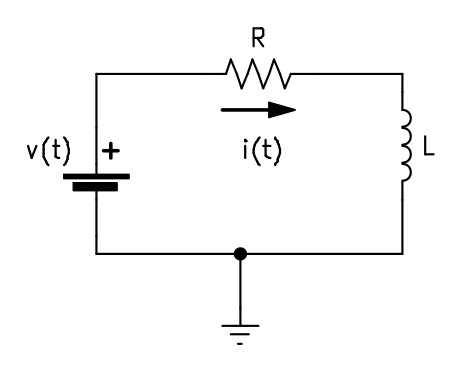
\includegraphics[width=0.5\textwidth]{RL_model}
    \caption{Electrical Model of a DC Motor}
    \label{fig:/Images/RL Circuit}
\end{figure}

Where $R$ is the winding resistance, $L$ is the winding inductance, $V(t)$ is the input voltage and $i(t)$ is the current through the coil winding. Using KVL we get
\begin{equation}
    v(t) = Ri(t) + L\frac{di}{dt}
\end{equation}
Taking the Laplace Transform
\begin{equation}
    V(s) = RI(s) + sLI(s)
\end{equation}
The transfer function is then
\begin{equation}
    \frac{I(s)}{V(s)} = H(s) = \frac{1}{sL+R}
\end{equation}
The system is converted from continuous time to discrete time by taking the zero-order hold equivalent. The zero-order hold equivalent to H(s) is defined by
\begin{equation}
    H_{h0}(z)= (1-z^{-1})\mathcal{Z}\{\frac{H(s)}{s}\}
\end{equation}
From (8) and (9) and using partial fraction expansion we get
\begin{equation}
    \frac{H(s)}{s} = \frac{1}{s(sL+R)} = \frac{1}{Rs} - \frac{L}{R(Ls+R)}
\end{equation}
We take the $\mathcal{Z}$-transform on (10) 
\begin{equation}
    \mathcal{Z}\{\frac{H(s)}{s}\} = \mathcal{Z}\{\frac{1}{Rs}\} - \mathcal{Z}\{\frac{L}{R(Ls+R)}\}
\end{equation}
Where the $z$-Transforms from above can be found using a $z$-transform table:
\begin{equation}
    \frac{1}{s} = \frac{z}{z-1}
\end{equation}
\begin{equation}
    \frac{1}{s+a} = \frac{z}{z-e^{-aT}}
\end{equation}
Using (12) and (13) the zero-order hold is expressed as
\begin{equation}
    H_{h0}(z) = (\frac{z-1}{z})\mathcal{Z}\{\frac{H(s)}{s}\} = (\frac{z-1}{z})\frac{1}{R}\left[ \frac{z}{z-1} - \frac{z}{z-e^{-\frac{R}{L}}T} \right]
\end{equation}
Then the expression simplifies to
\begin{equation}
    H_{h0}(z) = \frac{1}{R}\left[ \frac{1-e^{-\frac{R}{L}T}}{z-e^{-\frac{R}{L}T}} \right]
\end{equation}
Where $T$ is the sampling time. Below is the step response of the system for $R =0.362\Omega$, $L=567 \mu H$, and $T=25\mu s (e.g. 1/40kHz)$.

\begin{figure}[ht]
    \centering
    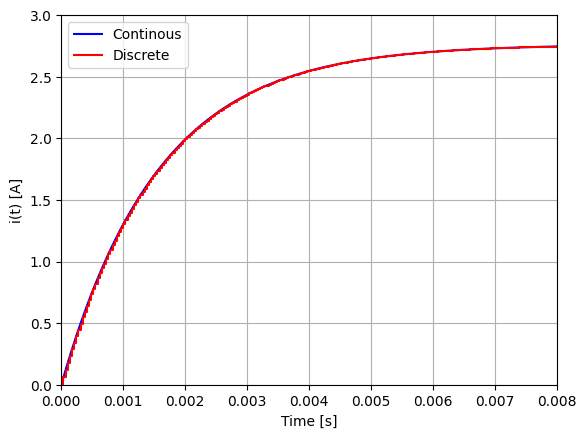
\includegraphics[width=0.5\textwidth]{c_v_d}
    \caption{Step Response}
    \label{fig:/Images/Step Response}
\end{figure}

Below is the bode plot of the plant. The system behaves as a low pass filter with a cutoff frequency of $\approx $ 0.02 radians per sample expressed by
\begin{equation}
    f_c =  1-e^{-\frac{RT}{L}}
\end{equation}
Note that the phase reaches -180 degrees at $\pi$ radians per sample

\begin{figure}[ht]
    \centering
    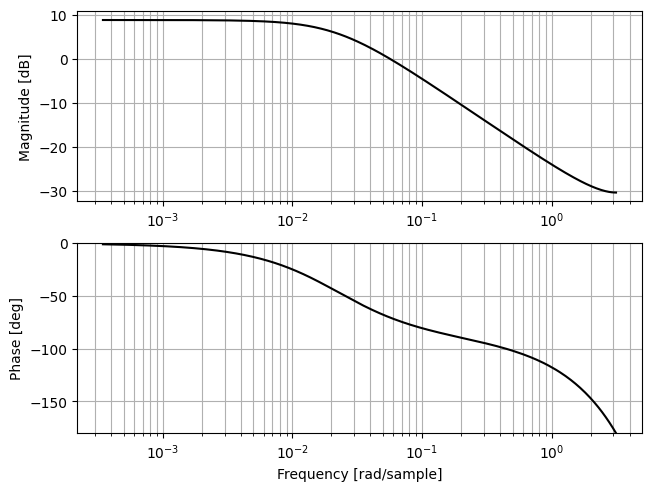
\includegraphics[width=0.5\textwidth]{bode_plot_plant}
    \caption{Plant Bode Plot}
    \label{fig:/ImagesPlant Bode Plot}
\end{figure}


\begin{tikzpicture}
    \centering
    \begin{semilogxaxis}[
    xlabel={Frequency (Hz)},
    ylabel={Magnitude (dB)},
    xmajorgrids=true,
    xminorgrids=true,
    ymajorgrids=true,
    ymajorgrids=true,legend pos=south west
    ]
    \addplot[black] table[x=freq_hz,y=mag_db,col sep=comma]{./Data/plant.csv};
    \addplot[red] table[x=freq_hz,y=mag_db,col sep=comma]{./Data/controller.csv};
    \addplot[green] table[x=freq_hz,y=mag_db,col sep=comma]{./Data/forward_path.csv};
    \addplot[blue] table[x=freq_hz,y=mag_db,col sep=comma]{./Data/closed_loop.csv};
    \addlegendentry{Plant}\addlegendentry{Controller}\addlegendentry{Foward Path}\addlegendentry{Closed Loop}
    %\addplot{x^2};
    \end{semilogxaxis}
\end{tikzpicture}
\begin{tikzpicture}
    \centering
    \begin{semilogxaxis}[
    xlabel={Frequency (Hz)},
    ylabel={Phase (deg)},
    xmajorgrids=true,
    xminorgrids=true,
    ymajorgrids=true,legend pos=south west
    ]
    \addplot[black] table[x=freq_hz,y=phase_deg,col sep=comma]{./Data/plant.csv};
    \addplot[red] table[x=freq_hz,y=phase_deg,col sep=comma]{./Data/controller.csv};
    \addplot[green] table[x=freq_hz,y=phase_deg,col sep=comma]{./Data/forward_path.csv};
    \addplot[blue] table[x=freq_hz,y=phase_deg,col sep=comma]{./Data/closed_loop.csv};
    \addlegendentry{Plant}\addlegendentry{Controller}\addlegendentry{Foward Path}\addlegendentry{Closed Loop}
    %\addplot{x^2};
    \end{semilogxaxis}
\end{tikzpicture}


\subsection{Controller Design}

A discrete time parallel PI controller is expressed by
\begin{equation}
    \frac{U(z)}{E(z)} = k\left( 1+\frac{k_i}{z-1}\right)
\end{equation}
where U is the controller effort, E is the error signal, 

\begin{equation}
    K_{p} = \frac{R_d \omega_c}{1-e^{\frac{-R_d T_s}{L_d}}}
\end{equation}

\begin{equation}
    K_{i} = 1-e^{\frac{-R_d T_s}{L_d}}
\end{equation}
Where $T_s = 1/40000$ is the sampling period [sec], $\omega_c = \pi/200$ is the cross-over frequency in rads/samples, $R_d = 0.362\Omega$, and $L_d = 567 \mu H$. $R_d$ and $L_d$ are the resistance and inductance of the d-axis circuit, respectively.\newline

The gains corresponding to a sampling frequency of 30kHz are P = 0.27005 and I = 0.021057, for the proportional and integral term, respectively. The D-axis current target is set to zero in order to maximize the torque per amp, so the q-axis current target is the only input to the controller.

A 1kHz PD impedance controller is wrapped around the current controller to implement a virtual spring and damper. The gains for the PD controller are P = 0.15 and D = 0.009, and these were determined experimentally by testing different values and inspecting the step response of the system.

\vspace{5mm} %5mm vertical space

\section{Motor Characterization}
\subsection{Torque Constant or Back EMF Constant ($K_T$ or $K_E$)}

To estimate this motor parameter, one needs to spin the motor with a drill and measure the peak-to-peak voltage ($V_{pk-pk}$) and the electrical frequency ($\omega_{el}$) with an oscilloscope on two of the three motor leads. The equation is

\begin{equation}
    K_{T} = \frac{0.5\times V_{pk-pk}}{\sqrt{2}\times2\pi\times\omega_{el}/NPP}
\end{equation}

The figure below illustrates the waveform generated and the corresponding measurements of the peak-to-peak voltage of 4.48V and electrical frequency of 59.97Hz, the number of pole pairs per rotation (NPP) is 7, so $K_T$ = 0.025 $\frac{Nm}{A}$. This parameter is important since it will be used to implement torque control.

\begin{figure}[h]

\begin{subfigure}{0.5\textwidth}
\includegraphics[width=0.9\linewidth, height=6cm]{V_pkpk} 
\caption{$V_{pk-pk}$}
\label{fig:subim1}
\end{subfigure}
\begin{subfigure}{0.5\textwidth}
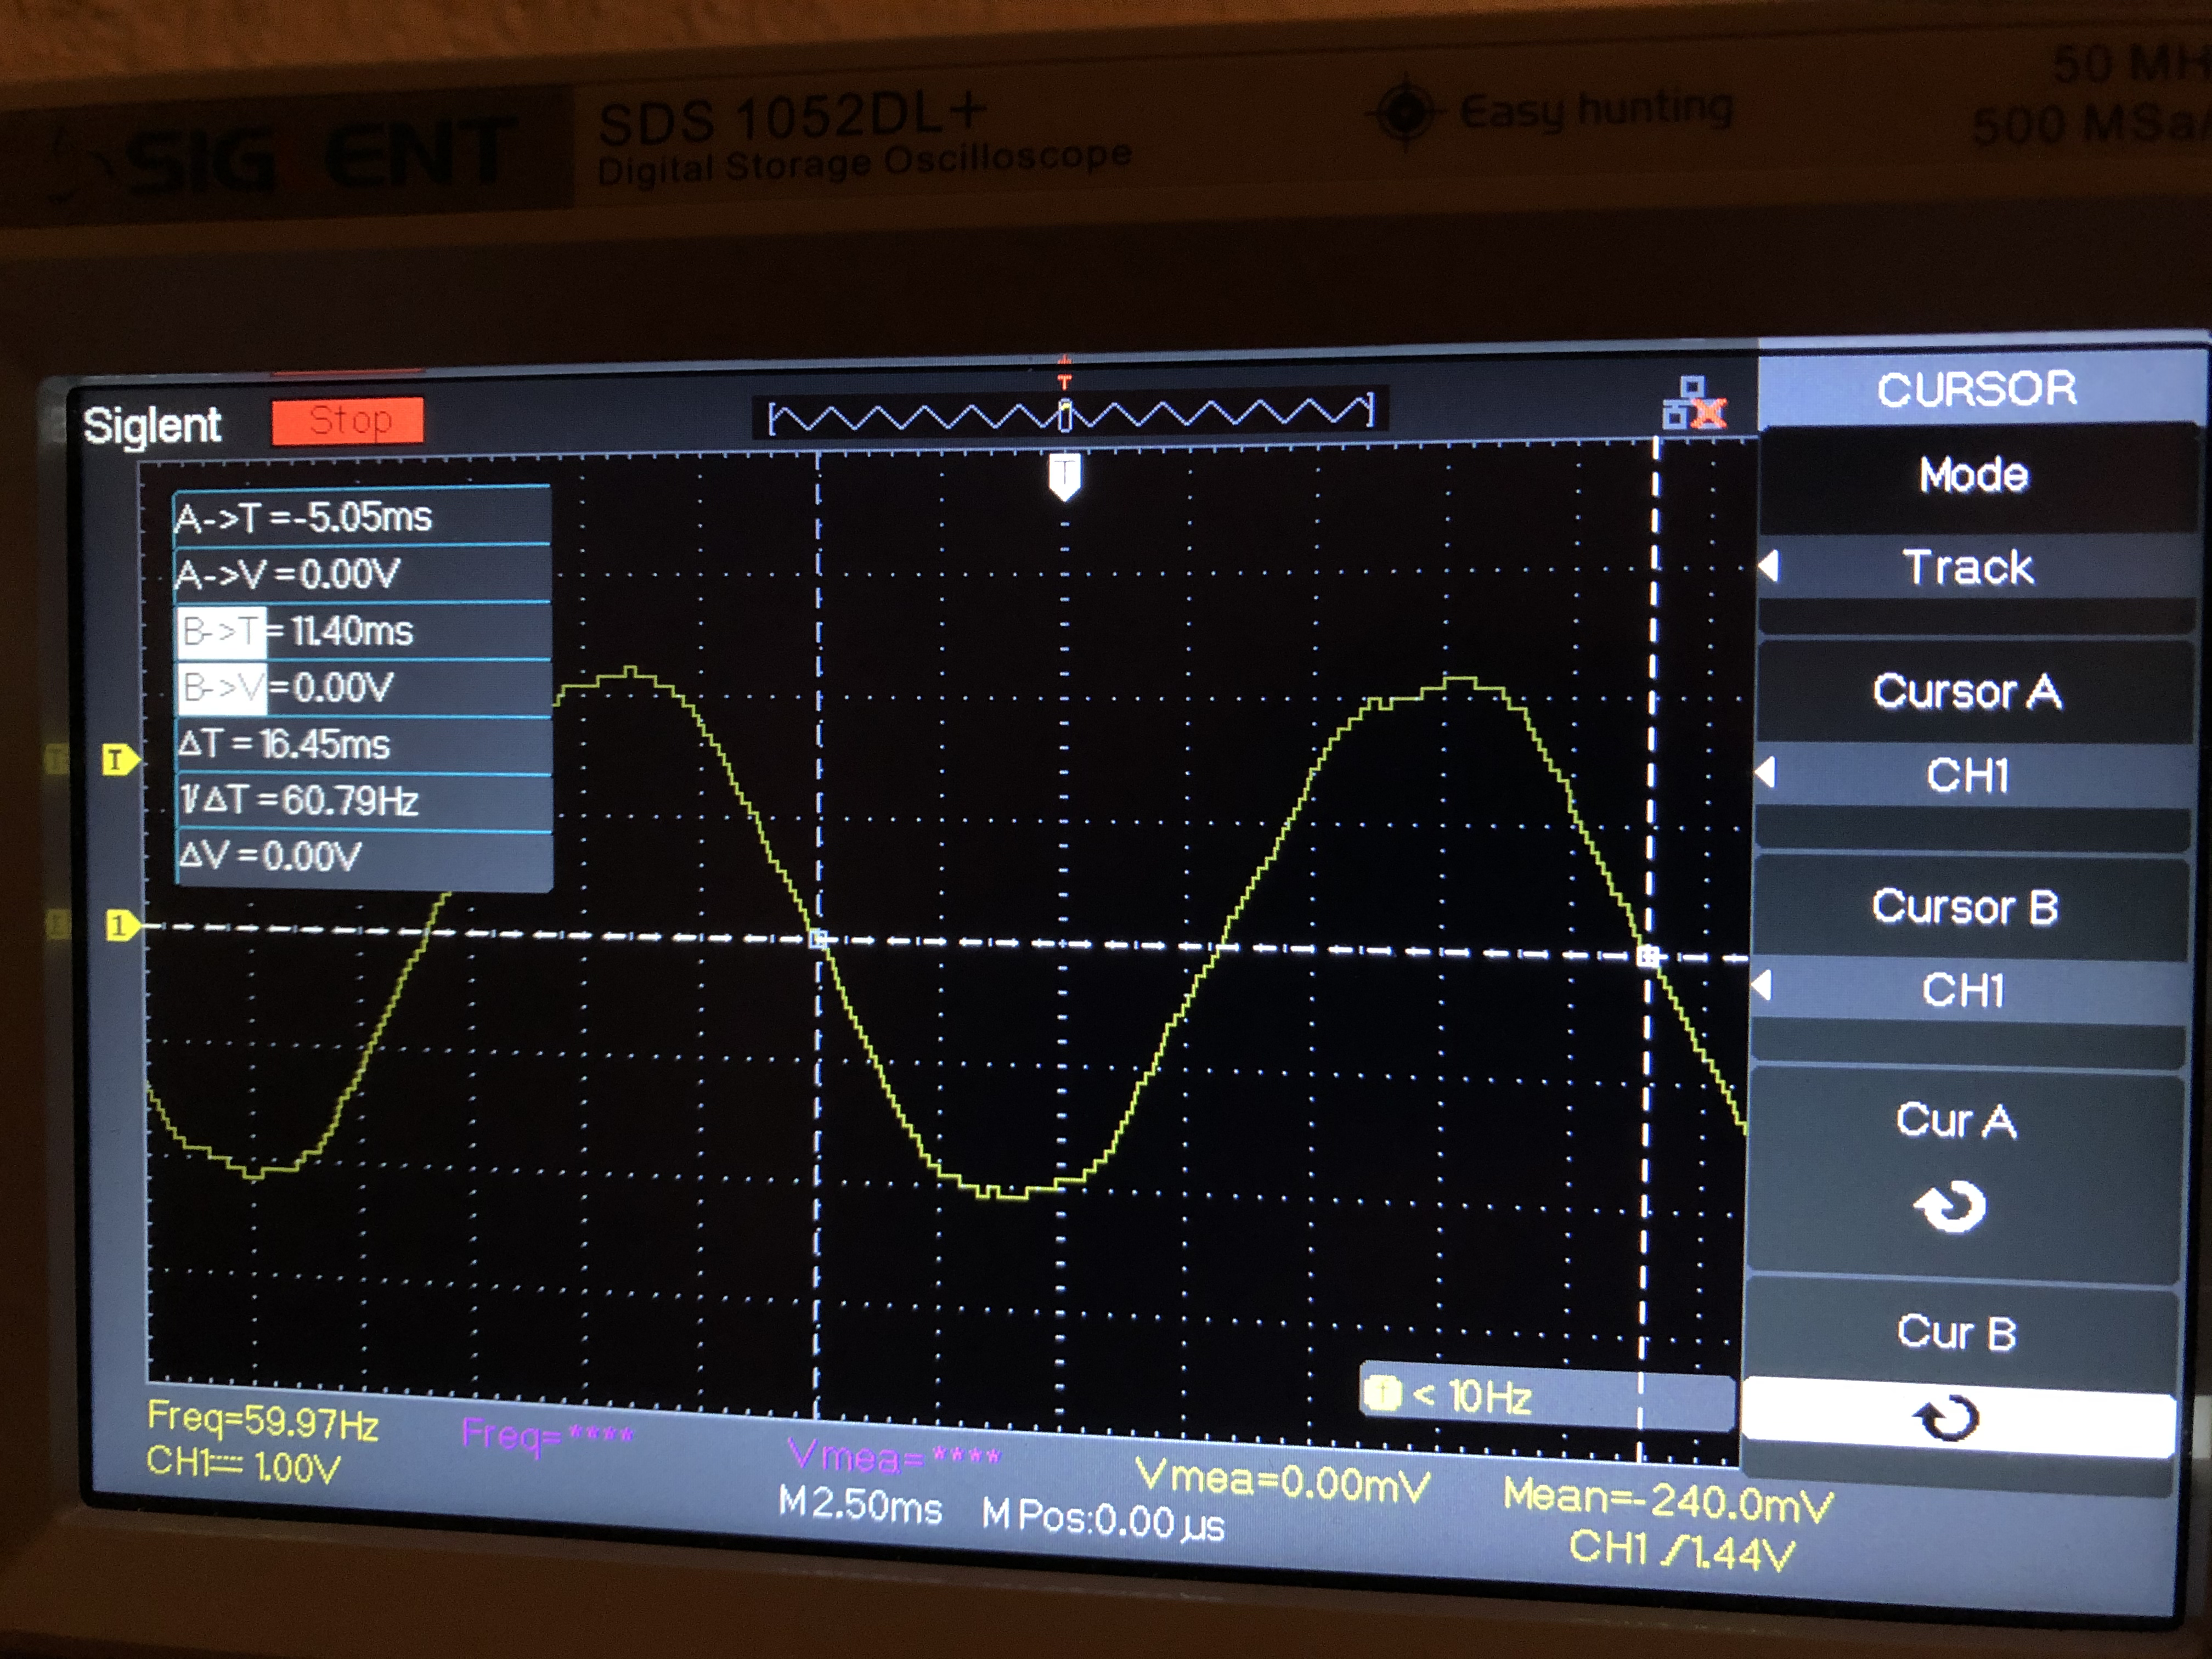
\includegraphics[width=0.9\linewidth, height=6cm]{w_el}
\caption{$\omega_{el}$}
\label{fig:subim2}
\end{subfigure}

\caption{Back EMF Measurement}
\label{fig:/Images/image2}
\end{figure}

\newpage

\subsection{Resistance and Inductance}

The motor resistance and inductance are needed in order to implement the PI current loops for the d-axis ($i_d$) and q-axis ($i_q$). These two parameters were measured by sending a step voltage of 0.2V through the d-axis and measuring the $i_d$ transient response with a DAC and an oscilloscope. The figure below illustrates the response and the fitted exponential model for comparison. 

\begin{figure}[ht]
    \centering
    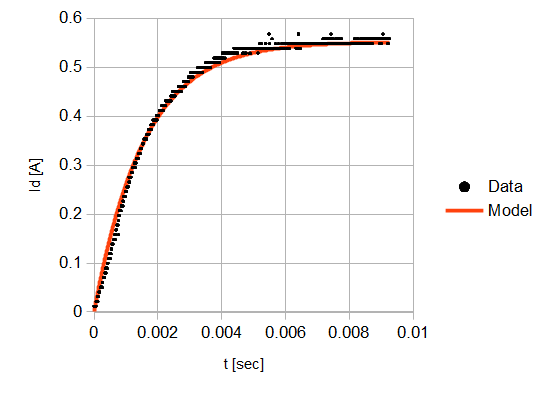
\includegraphics[width=0.5\textwidth]{RL_Step_Response_Id}
    \caption{Step Response of RL Circuit}
    \label{fig:/Images/RL_Step_Response_Id}
\end{figure}

The resistance was estimated using Ohm's law during the steady state part of the response ($v_d/i_d$ = 0.2V/0.553A = 0.362$\Omega$). Once we know the resistance, we use the transient part of the response to estimate the inductance of 567uH. We find the time constant ($\tau$) by inspecting how much time it takes the current to reach 63.2$\%$ from it's steady state value which was 1.57ms. Then the inductance can be calculated using the following equation 

\begin{equation}
    \tau = \frac{L_d}{R}
\end{equation}

Note that for PMSM the d-axis and q-axis inductance are quite similar, so for simplicity we can let $L_d = L_q$ in order to use the same set of gains for each of the PI current loops.

\subsection{Rotor Inertia and Viscous Damping}

The viscous damping ($b$ = 8.4E-5 Nm.s/rad)was estimated by solving for the linear viscous term when running the motor at constant voltage (Vq) input and constant velocity by using the following expression:

\begin{equation}
    J\ddot{\theta} + b\dot{\theta}= K_Ti = \frac{KV_Q-K_T^2\dot{\theta}}{R}
\end{equation}
\begin{equation}
    b = \frac{KV_Q-K_T^2\dot{\theta}}{\dot{\theta}R}
\end{equation}

The rotor inertia ($J$ = 4.0102e-07 kg·m²) was estimated by applying a step voltage to the q-axis and measuring the transient response of the velocity. The figure below illustrates the response and the fitted exponential model for comparison.

\begin{figure}[ht]
    \centering
    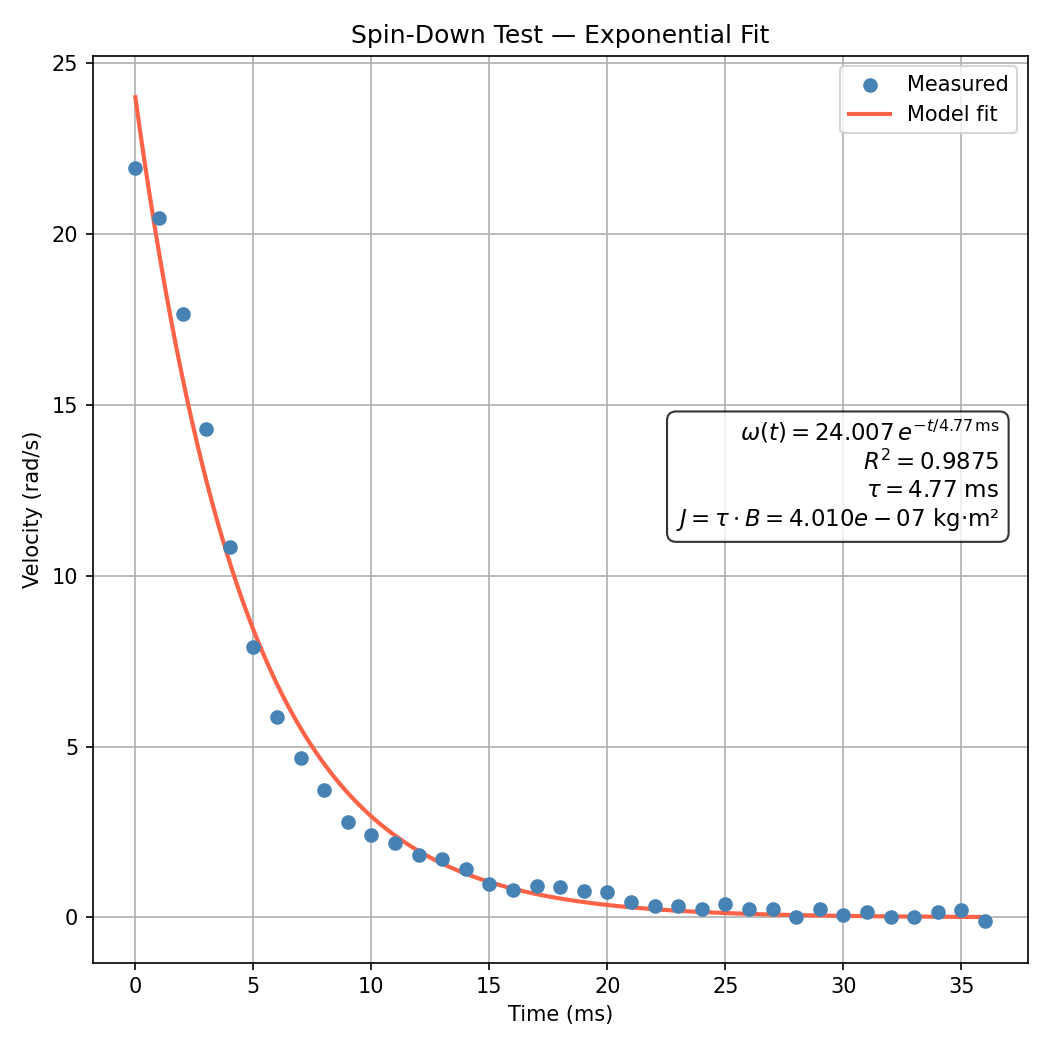
\includegraphics[width=0.5\textwidth]{spin_down_fit}
    \caption{Step Response of Motor Velocity}
    \label{fig:/Images/spin_down_fit}
\end{figure}

For position control, Kp gain was determined experimentally and a value of 0.15 works well with a Kd gain 0.009

Now that the motor has been characterized, simulations were ran t generate the torque speed curve and efficienty map.

\begin{figure}[ht]
    \centering
    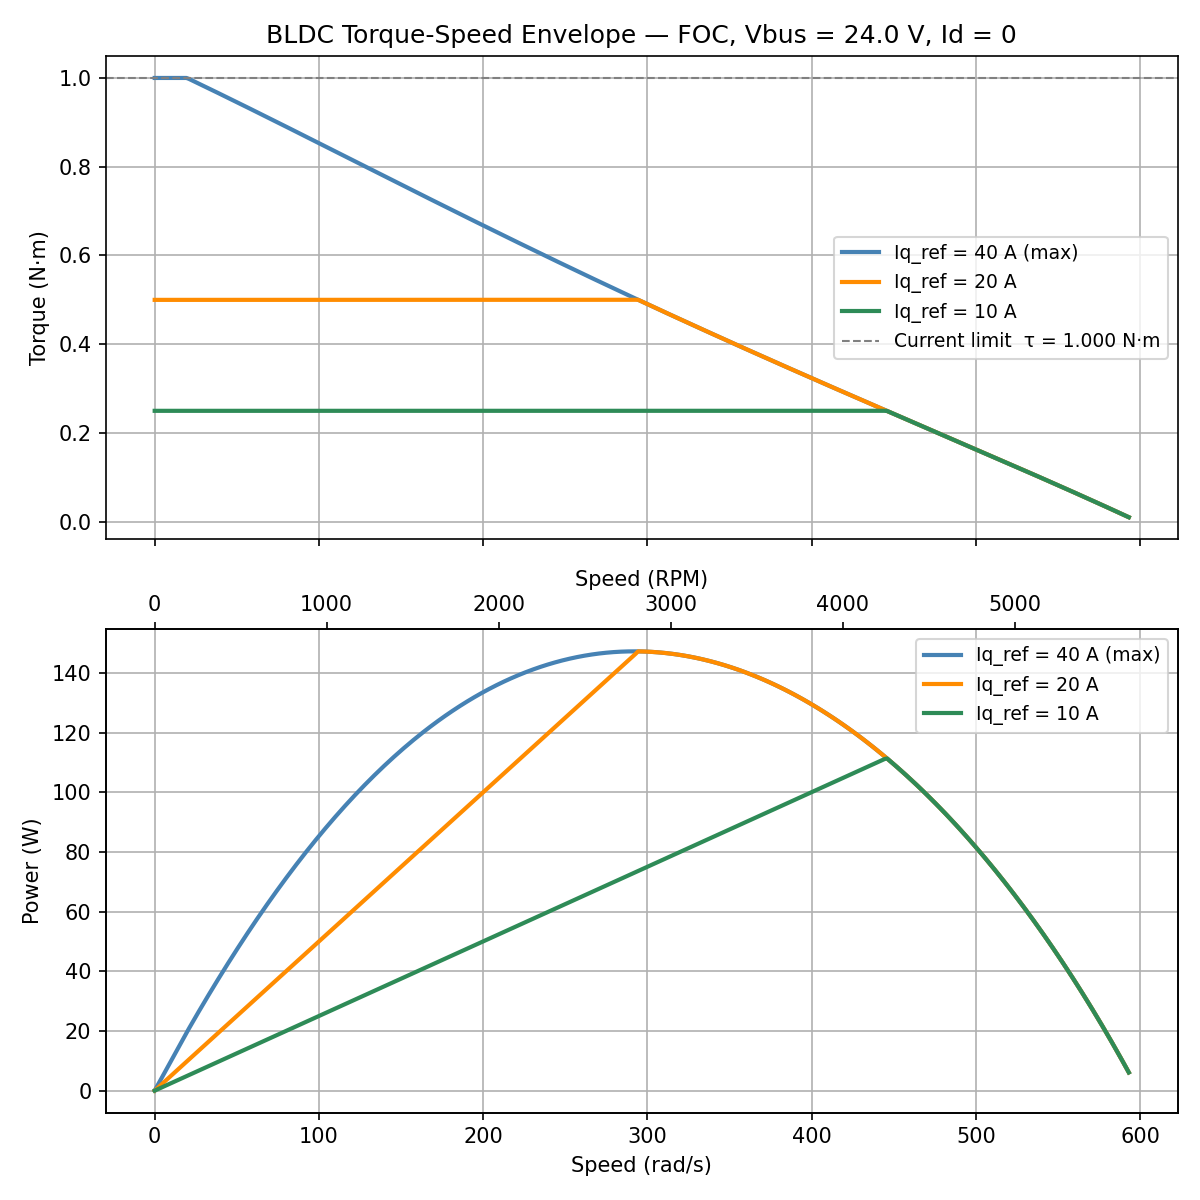
\includegraphics[width=0.5\textwidth]{torque_speed}
    \caption{Torque-Speed Characteristic}
    \label{fig:/Images/torque_speed}
\end{figure}

\begin{figure}[ht]
    \centering
    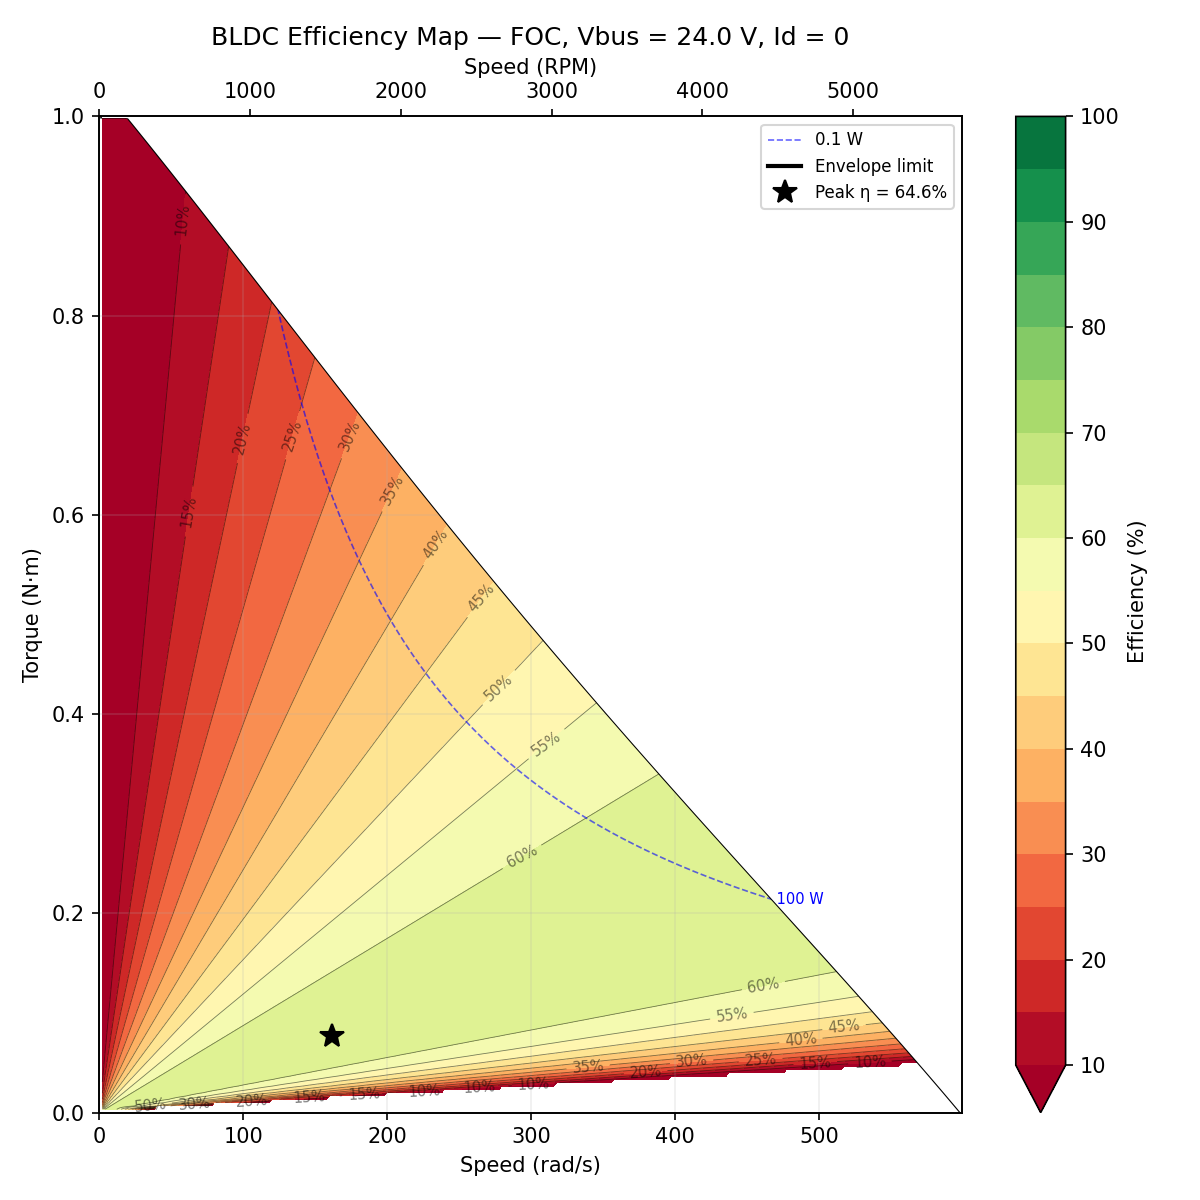
\includegraphics[width=0.5\textwidth]{efficiency_map}
    \caption{Efficiency Map}
    \label{fig:/Images/efficiency_map}
\end{figure}

\begin{comment}
\end{comment}
\end{document}